\chapter{Unified Process (UP)}

\section{OOA e OOD}

\dfn{OOA/D}{
    \begin{itemize}
        \item \textbf{OOA} (Object Oriented Analysis): studio dei requisiti e delle specifiche del sistema;
        \item \textbf{OOD} (Object Oriented Design): progettazione del sistema.
    \end{itemize}

    Per studiare OOA/D si utilizza Unified Process, 
    un processo di sviluppo software orientato agli oggetti.
}

\nt{UP può essere applicato usando un 
approccio agile come Scrum o XP.}

\cor{UML}{
    UP utilizza UML come linguaggio di modellazione.
    UML è un linguaggio di modellazione grafico e testuale
    per la specifica, la costruzione e la documentazione
    di sistemi software orientati agli oggetti.

    \paragraph{IMPORTANTE:} UML non è nato per descrivere software, ma
    per descrivere concetti\footnote{Simile a ER, visto nel corso "Basi di dati".}.
}

\subsubsection{OOD è guidata dalle responsabilità (si vedano
i pattern GRASP):}

\begin{itemize}
    \item [$\Rightarrow$] Quali sono gli oggetti? Quali sono le classi?
    \item [$\Rightarrow$] Cosa deve conoscere un oggetto? Cosa deve saper fare?
    \item [$\Rightarrow$] Come collaborano gli oggetti?
\end{itemize}

\dfn{Pattern}{
    I pattern sono euristiche, best practice, che aiutano a codificare principi
    di soluzioni.
}


\subsubsection{ODD è correlata all'analisi dei requisiti:}

\begin{itemize}
    \item [$\Rightarrow$] \fancyglitter{Casi d'uso};
    \item [$\Rightarrow$] \fancyglitter{Storie utente}.
\end{itemize}
\pagebreak
\ex{Gioca una \newfancyglitter{partita a dadi}}{
\subsubsection{Definizione dei casi d'uso: storie scritte.}

Il \newfancyglitter{Giocatore} chiede
di \fancyglitter{lanciare} i \newfancyglitter{dadi}. Il Sistema presenta il
\fancyglitter{risultato}: se \fancyglitter{il valore totale} delle facce dei dadi
è sette, il giocatore ha vinto; altrimenti ha
perso.

\subsubsection{Definizione di un modello di dominio:
\newfancyglitter{i concetti o gli oggetti significativi}.}

\begin{center}
    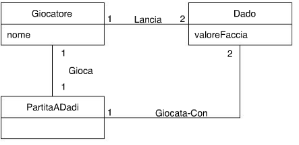
\includegraphics[scale=0.7]{images/Dadi.png}
\end{center}

\subsubsection{Assegnare responsabilità agli oggetti e 
disegnare diagrammi di interazione: \fancyglitter{responsabilità e collaborazioni}.}

\begin{center}
    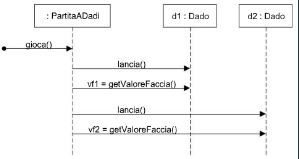
\includegraphics[scale = 0.7]{images/Dadi2.png}
\end{center}

\subsubsection{Definizione dei diagrammi delle classi di progetto.}

\begin{center}
    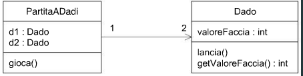
\includegraphics[scale=0.7]{images/Dadi 3.png}
\end{center}

}
\subsubsection{}
L'analisi dei requisiti e l'OOA/D vanno svolte nel contesto di un processo di sviluppo:

\begin{itemize}
    \item [$\Rightarrow$] Sviluppo iteratuivo;
    \item [$\Rightarrow$] Approccio agile;
    \item [$\Rightarrow$] Unified Process (UP).
\end{itemize}

\nt{ER e UML non sono pienamente adatti a possibili incrementi.}
\pagebreak

\subsection{UML}

\dfn{UML}{UML è un linguaggio \newfancyglitter{visuale} per la specifica,
la costruzione e la documentazione degli elaborati di un sistema software.

UML è uno standard per la notazione di diagrammi per disegnare o rappresentare
figure relative al software (specialmente OO).}
\subsubsection{}
UML è un \textit{abbozzo} o un \textit{progetto} per aiutare la comprensione nei team di sviluppo.
Il termine abbozzo indica che può essere soggetto a correzzione, ma se non ci 
sono feedback a tal proposito deve essere trattato come un dizionario.

\subsubsection{Uso di UML:}

\begin{itemize}
    \item [$\Rightarrow$] Punto di vista \fancyglitter{concettuale}: modello 
    di dominio, per visualizzare concetti del mondo reale;
    \item [$\Rightarrow$] Punto di vista \fancyglitter{software}: diagramma
    delle classi di progetto, utilizzata per visualizzare elementi software.
\end{itemize}

\subsubsection{Brevi note storiche:}

\begin{itemize}
    \item [$\Rightarrow$] Anni '60 e '70: nascita dei linguaggi OO (Simula e Smalltalk);
    \item [$\Rightarrow$] 1988: Bertrand Meyer, "Object-Oriented Software";
    \item [$\Rightarrow$] 1991: Jim Rumbaugh, "Object-Oriented Modelling and Design" (OOA/D);
    \item [$\Rightarrow$] 1991, Grady Booch, "Object-Oriented Software Engineering" (OOA/D e Casi d'Uso);
    \item [$\Rightarrow$] 1994, Rumbaugh e Booch fanno le prime proposte di UML;
    \item [$\Rightarrow$] Rational Corporation fondata dai "tre amigos" (Jacobson, Booch e Rumbaugh);
    \item [$\Rightarrow$] 1997 UML 1;
    \item [$\Rightarrow$] 2004 UML 2 (usato attualmente).
\end{itemize}

\section{Unified Process}

\dfn{Unified Process}{
    Unified Process è un processo iterativo ed evolutivo (incrementale)
    per lo sviluppo del software per la costruzione di sistemi orientati agli oggetti.
    Le iterazioni iniziali sono guidate dal \newfancyglitter{rischio}, dal
    \newfancyglitter{cliente} e dall'\newfancyglitter{architettura}.
}

\qs{}{Cosa c'è in UP?}

\begin{itemize}
    \item [$\Rightarrow$] Un'organizzazione del piano di progetto
    per fasi sequenziali;
    \item [$\Rightarrow$] Indicazioni sulle attività da svolgere nell'ambito
    di discipline e sulle loro inter-relazioni;
    \item [$\Rightarrow$] Un insieme di ruoli predefiniti;
    \item [$\Rightarrow$] Un insieme di artefatti da produrre.
\end{itemize}

\subsubsection{Un progetto UP è organizzato in 4 fasi:}

\begin{itemize}
    \item [$\Rightarrow$] \fancyglitter{Ideazione} (inception): visione approssimativa, studio economico, portata, stime approssimative di costi e tempi. \textbf{\underline{Milestone}:} \newfancyglitter{Obiettivi};
    \item [$\Rightarrow$] \fancyglitter{Elaborazione} (elaboration): visione raffinata, implementazione iterativa del nucleo dell'architettura, risoluzione dei rischi maggiori, identificazione della maggior parte dei requisiti e della portata, stime più realistiche sulle loro inter-relazioni. \textbf{\underline{Milestone}:} \newfancyglitter{Architetturale};  
    \item [$\Rightarrow$] \fancyglitter{Costruzione} (construction): implementazione iterativa degli elementi rimanenti, più facili e a rischio minore, preparazione al rilascio. \textbf{\underline{Milestone}:} \newfancyglitter{Capacità operazionale};
    \item [$\Rightarrow$] \fancyglitter{Transizione} (transition): beta test, rilascio. \textbf{\underline{Milestone}:} \newfancyglitter{Rilascio prodotto}.
\end{itemize}

\begin{center}
    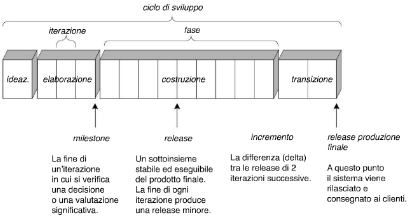
\includegraphics[scale = 1]{images/UP.png}
\end{center}

\nt{
    \begin{itemize}
        \item [$\Rightarrow$] L'Ideazione non è una fase di requisiti, ma di fattibilità;
        \item [$\Rightarrow$] L'Elaborazione non è una fase di requisiti o di progettazione, ma una fase in cui 
        si implementa in modo iterativo l'architettura del sistema e vengono ridotti i rischi maggiori.
    \end{itemize}
}

\subsection{Le discipline}

\dfn{Discipline}{
    Una disciplina è un insieme di attività e dei relativi \newfancyglitter{elaborati}
    in una determinata area, come le attività relative all'analisi dei requisiti. 
}

\cor{Elaborato}{
    Un elaborato (artefatto o work product) è il termine generico che indica un qualsiasi prodotto di lavoro: codice, schemi di basi di dati, 
    documenti di testo, diagrammi, modelli, etc.
}

\subsubsection{Discipline ingegneristiche di UP:}

\begin{itemize}
    \item [$\Rightarrow$] \fancyglitter{Modellazione del business}: attività che 
    modellano il dominio del problema e il suo ambito;
    \item [$\Rightarrow$] \fancyglitter{Requisiti}: attività di raccolra dei requisiti;
    \item [$\Rightarrow$] \fancyglitter{Progettazione} (analysis and design): attività di analisi dei requisiti
    e progetto architetturale;
    \item [$\Rightarrow$] \fancyglitter{Implementazione}: attività di progetto dettagliato e codifica del sistema, test sui componenti;
    \item [$\Rightarrow$] \fancyglitter{Test}: attività di controllo di qualità, test di integrazione e di sistema;
    \item [$\Rightarrow$] \fancyglitter{Rilascio}: attività di consegna e messa in opera.
\end{itemize}

\subsubsection{Discipline di supporto di UP:}

\begin{itemize}
    \item [$\Rightarrow$] \fancyglitter{Gestione delle configurazioni e del cambiamento}: attività di manutenzione durante il progetto;
    \item [$\Rightarrow$] \fancyglitter{Gestione progetto}: attività di pianificazione e governo del progetto;
    \item [$\Rightarrow$] \fancyglitter{Infrastruttura} (enviroment): attività che supportano il team di progetto, riguardo ai processi e strumenti utilizzati.
\end{itemize}

\nt{Nonostante le fasi siano \newfancyglitter{sequenziali}, le discipline non lo sono (perchè si eseguono in ogni iterazione).
Il numero di iterazioni dipende dal Project Manager.}

\subsubsection{Uso di UML in UP:}

\begin{itemize}
    \item [$\Rightarrow$] UP usa solo UML come linguaggio di modellazione;
    \item [$\Rightarrow$] I diagrammi UML si usano con variabilità, bisogna \newfancyglitter{personalizzare} UP;
    \item [$\Rightarrow$] I diagrammi si usano in UP seguendo le iterazioni e gli incrementi;
    \item [$\Rightarrow$] UP dice \newfancyglitter{quando} usare un diagramma;
    \item [$\Rightarrow$] In UP quasi tutto è \newfancyglitter{opzionale} eccetto che lo sviluppo iterativo e guidato dal rischio, la verifica continua della qualità e il codice;
    \item [$\Rightarrow$] La scelta delle pratiche e degli artefatti UP si riassume in un documento (\newfancyglitter{scenario di sviluppo}).
\end{itemize}

\subsection{Che cosa sono i requisiti?}

\dfn{Requisito}{
    Un requisito è una \newfancyglitter{capacità} o una condizione a cui il sistema deve essere \newfancyglitter{conforme}.
}

\cor{Sorgenti dei requisiti}{
    I requisiti derivano da richieste degli utenti del sistema per risolvere dei problemi e raggiungere degli obiettivi.
    Possono essere:
    \begin{itemize}
        \item [$\Rightarrow$] \fancyglitter{Requisiti funzionali}: descrivono il comportamento del sistema in termini di funzionalità offerte;
        \item [$\Rightarrow$] \fancyglitter{Requisiti non funzionali}: le proprietà del sistema nel suo complesso (sicurezza, prestazioni, etc.).
    \end{itemize}
}

\nt{
    In UP bisogna gestire i requisiti: si utilizza un approccio sistematico
    per trovare, documentare, organizza e tracciare i \underline{requisiti che cambiano}
    di un sistema. Si inizia a programmare quando sono stati specificati il 10\% o il 20\%
    dei requisiti significativi.
}

\subsubsection{Acquisizione sistematica dei requisiti:}

\begin{itemize}
    \item [$\Rightarrow$] Scrivere i Casi d'Uso con i clienti;
    \item [$\Rightarrow$] Workshop dei requisiti con sviluppatori e clienti;
    \item [$\Rightarrow$] Gruppi di lavoro con rappresentanti dei clienti;
    \item [$\Rightarrow$] Dimostrazione ai clienti dei risultati di ciascuna iterazione, per favorire un feedback.
\end{itemize}

\subsubsection{Modello FURPS+:}

\begin{itemize}
    \item [$\Rightarrow$] \fancyglitter{Funzionali} (F): requisiti funzionali e di sicurezza;
    \item [$\Rightarrow$] \fancyglitter{Usabilità} (U): facilità d'uso del sistema;
    \item [$\Rightarrow$] \fancyglitter{Affidabilità} (R - Reliability): disponibilità del sistema, capacità di tollerare guasti o di essere ripristinato;
    \item [$\Rightarrow$] \fancyglitter{Prestazioni} (P): tempi di risposta, throughput, capacità e uso delle risorse;
    \item [$\Rightarrow$] \fancyglitter{Sostenibilità} (S): facilità di modifica per riparazioni e miglioramenti, adattabilità, manutenibilità, localizzazione, configurazione, compatibilità;
    \item [$\Rightarrow$] \fancyglitter{+}: vincoli di progetto, interoperabilità, operazionali, fisici, legali, etc.
\end{itemize}

\subsubsection{Elaborati:}

\begin{itemize}
    \item [$\Rightarrow$] \fancyglitter{Modello dei Casi d'Uso}: scenari tipi dell'utilizzo di un sistema;
    \item [$\Rightarrow$] \fancyglitter{Specifiche supplementari}: ciò che non rientra nei Casi d'Uso, requisiti non funzionali o funzionali non esprimibili attraverso i Casi d'Uso;
    \item [$\Rightarrow$] \fancyglitter{Glossario}: termini significativi, dizionario dei dati;
    \item [$\Rightarrow$] \fancyglitter{Visione}: riassume i requisiti di alto livello, un documento sintetico per apprendere rapidamente le idee principali del progetto;
    \item [$\Rightarrow$] \fancyglitter{Regole di Business}: regole di dominio, i requisiti o le politiche che trascendono un unico progetto software e a cui un sistema deve conformarsi.
\end{itemize}

\section{Ideazione}

\qs{}{Che cos'è l'ideazione?}

\paragraph{Risposta:} l'ideazione permette di stabilire una visione completa
e la portata del progetto (\newfancyglitter{studio di fattibilità}).

\subsubsection{Durante l'ideazione:}

\begin{itemize}
    \item [$\Rightarrow$] Si analizzano il 10\% dei Casi d'Uso;
    \item [$\Rightarrow$] Si analizzano i requisiti non funzionali più importanti;
    \item [$\Rightarrow$] Si realizza una stima dei costi;
    \item [$\Rightarrow$] Si prepara l'ambiente di sviluppo;
    \item [$\Rightarrow$] \newfancyglitter{Durata:} breve.
\end{itemize}

\nt{Lo scopo dell'Ideazione \underline{non} è di raccogliere tutti i requisiti, né di generare
una stima o un piano di progetto affidabile.
Durante l'ideazione si cerca di capire se il progetto è fattibile e se ha senso.}

\definecolor{dkgreen}{rgb}{0, 0.5, 0}
\definecolor{mgray}{rgb}{0.9, 0.9, 0.9}
\begin{center}
    \begin{tabular}{ || >{\columncolor{mgray}}p{8cm} | >{\columncolor{GreenPastel}}p{8cm} ||}
    \hline\hline
        \rowcolor{lightgray}
    \textbf{Elaborato}& \textbf{\textcolor{dkgreen}{Commento}}\\ \hline
    \hline
        Visione e studio economico & Descrive obiettivi e vincoli di alto livello, fornisce un sommario del progetto.\\ \hline

        Modello dei Casi d'Uso & Descrive i requisiti funzionali del sistema. Vengono identificati i nomi della maggior parte dei Casi d'Uso.\\ \hline

        Specifiche supplementari & Descrive i requisiti non funzionali e i requisiti funzionali non esprimibili attraverso i Casi d'Uso.\\ \hline

        Glossario & Definisce i termini significativi del dominio.\\ \hline

        Lista dei Rischi e Piano di Gestione dei Rischi & Identifica i rischi principali e come affrontarli.\\ \hline

        Prototipi e proof of concept & Dimostrano la fattibilità tecnica e la comprensione dei requisiti.\\ \hline

        Piano dell'Iterazione & Fornisce una descrizione di cosa fare nella prima iterazione dell'elaborazione.\\ \hline

        Piano delle Fasi e Piano di Sviluppo del Software & Ipotesi (poco precise) riguardo la fase di elaborazione.\\ \hline 
    
        Scenario di Sviluppo & Descrive le pratiche e gli artefatti UP da usare.\\ \hline
    
        \hline

    \end{tabular}
\end{center}

\subsection{Artefatti nell'Ideazione}

\qs{}{La documentazione non è troppa?}

\paragraph{Risposta:} lo scopo della documentazione non è nel documento in sè, ma nel pensare:

\begin{itemize}
    \item [$\Rightarrow$] gli artefatti sono quelli che aggiungono valore;
    \item [$\Rightarrow$] sono parzialmente completati;
    \item [$\Rightarrow$] sono preliminari e approssimativi.
\end{itemize}

\nt{Nessun documento è definitivo.}

\dfn{Specifiche supplementari}{
    Le \newfancyglitter{specifiche supplementari} raccolgono altri requisiti,
    informazioni e vincoli che non sono espressi nei Casi d'Uso o nel Glossario. 
    Si deve mettere anche la cronologia delle versioni.
}

\subsection{Tipologie di documenti}

\dfn{Visione}{
    Il documento \newfancyglitter{Visione} riassume alcune informazioni contenute nel modello dei Casi d'Uso e 
    nelle Specifiche supplementari. Inoltre descrive brevemente il progetto ai partecipanti per stabilire una
    visione comune.
    
    \begin{itemize}
        \item [$\Rightarrow$] Obiettivi e problemi fondamentali ad alto livello\footnote{Soprattutto per i requisiti non funzionali};
        \item [$\Rightarrow$] Riepilogo delle caratteristiche di sistema.
    \end{itemize}
}

\nt{Spesso è utile iniziare da un Glossario.}

\dfn{Glossario e dizionario dei dati}{
    Il \newfancyglitter{Glossario} è un documento che definisce i termini significativi del dominio e le relazioni tra di
    essi. Si devono eliminare eventuali discrepanze per ridurre problemi di comunicazione e di ambiguità.

    In UP il Glossario svolge anche il ruolo di \newfancyglitter{dizionario dei dati}:
    un documento di dati che si riferiscono ad altri dati\footnote{Metadati.}, per esempio le regole di validazione.
}

\cor{Regole di dominio}{
    Le \newfancyglitter{regole di dominio} (o regole di Business\footnote{Viste in "Basi di dati".}) stabiliscono
    come può funzionare un dominio o un business.

}


\section{Casi d'Uso}

\subsection{Disciplina dei requisiti}

\dfn{Disciplina dei requisiti}{
    La \newfancyglitter{disciplina dei requisiti} è il processo
    per scoprire cosa deve essere costruito e orientare lo sviluppo verso 
    il sistema corretto.
}

\cor{Requisiti di sistema}{
    I requisiti di sistema sono le capacità e le condizioni
    a cui il sistema deve essere conforme.
}

\nt{I requisiti di sistema sono scritti nel "linguaggio del cliente".}

\subsubsection{Passi principali:}

\begin{itemize}
    \item [$\Rightarrow$] Produrre una \fancyglitter{lista dei requisiti potenziali} (candidati);
    \item [$\Rightarrow$] Capire il \fancyglitter{contesto} del sistema;
    \item [$\Rightarrow$] Catturare i \fancyglitter{requisiti funzionali} (di comportamento);
    \item [$\Rightarrow$] Catturare i \fancyglitter{requisiti non funzionali}.
\end{itemize}

\subsubsection{Ogni requisito è caratterizzato da:}

\begin{itemize}
    \item [$\Rightarrow$] \fancyglitter{Breve descrizione};
    \item [$\Rightarrow$] \fancyglitter{Stato} (proposto, approvato, incorporato, validato);
    \item [$\Rightarrow$] \fancyglitter{Costi di implementazione stimati};
    \item [$\Rightarrow$] \fancyglitter{Priorità};
    \item [$\Rightarrow$] \fancyglitter{Rischio associato per la sua implementazione}.
\end{itemize}

\dfn{Lista dei requisiti}{
    La \newfancyglitter{lista dei requisiti} è usata per stimare la taglia del progetto e per
    decidere come suddividere il lavoro in sequenze di iterazioni.
}

\subsection{Capire il contesto del sistema e catturare i requisiti}

\subsubsection{Ci sono due modi per capire il contesto del sistema:}

\begin{itemize}
    \item [$\Rightarrow$] \fancyglitter{Modello di dominio}: descrive i concetti significativi del sistema come oggetti del dominio e relaziona i concetti con associazioni (usa UML);
    \item [$\Rightarrow$] \fancyglitter{Modello di business}: un super-insieme del modello di dominio, descrive i processi di business. È un prodotto dell'ingegneria del business e ha lo scopo di migliorare i processi di business. 
\end{itemize}

\nt{Il contesto del sistema è catturato dal \newfancyglitter{diagramma UML dei Casi d'Uso}.}

\subsubsection{Catturare i requisiti funzionali:}

\begin{itemize}
    \item [$\Rightarrow$] In UP vengono usati i Casi d'Uso;
    \item [$\Rightarrow$] Un Caso d'Uso rappresenta un possibile utilizzo del sistema da parte di un utente;
    \item [$\Rightarrow$] Sono descrizioni testuali.
\end{itemize}

\subsubsection{Catturare i requisiti non funzionali:}

\begin{itemize}
    \item [$\Rightarrow$] Si utilizzano le Specifiche supplementari;
    \item [$\Rightarrow$] Possono ancge essere catturati nei Casi d'Uso.
\end{itemize}

\subsection{Casi d'Uso e UP}

\subsubsection{UP è una metodologia "\fancyglitter{use-case driven}":}
\begin{itemize}
    \item [$\Rightarrow$] I Casi d'Uso si usano per pianificare le iterazioni;
    \item [$\Rightarrow$] L'analisi e la progettazione si basano sui Casi d'Uso;
    \item [$\Rightarrow$] I Casi d'Uso sono usati per definire i test;
    \item [$\Rightarrow$] I Casi d'Uso influiscono nella redazione dei manuali utente e della Visione;
    \item [$\Rightarrow$] \fancyglitter{Attori}: qualcosa o qualcuno dotato di \newfancyglitter{comportamento};
    \item [$\Rightarrow$] \fancyglitter{Scenario} (istanza di Caso d'Uso): \newfancyglitter{sequenza specifica di azioni e interazioni} tra l sistema e alcuni attori. Descrive una particolare storia;
    \item [$\Rightarrow$] \fancyglitter{Caso d'Uso}: \newfancyglitter{insieme di scenari} che descrivono un attore che usa il sistema per \newfancyglitter{raggiungere un obiettivo specifico}.
\end{itemize}

\nt{I Casi d'Uso possono essere di successo o di fallimento.

\paragraph{ATTENZIONE:} sono documenti di testo, non diagrammi.}
\pagebreak
\ex{Caso d'Uso: breve descrizione}{
    \begin{center}
        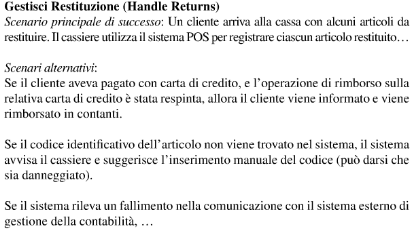
\includegraphics[scale = 0.7]{images/Gestisci restituzione.png}
    \end{center}

}

\dfn{Modello dei Casi d'Uso}{
    Il \newfancyglitter{modello dei Casi d'Uso} è un modello delle funzionalità del sistema. Include un diagramma
    UML dei Casi d'Uso che funge da \newfancyglitter{modello di contesto} del sistema e da \newfancyglitter{indice dei nomi} di Caso d'Uso.

}

\nt{I Casi d'Uso sono utili per rappresentare i requisiti come OOA/D.

I Casi d'Uso definiscono i \newfancyglitter{contratti} (vedi sezione \ref{contratti}) in relazione al comportamento del sistema.}


\subsubsection{L'enfasi è posta sull'utente:}
\begin{itemize}
    \item [$\Rightarrow$] Chi utilizza il sistema?
    \item [$\Rightarrow$] Quali sono i loro Scenari d'Uso tipici?
    \item [$\Rightarrow$] Quali sono i loro obiettivi?
    \item [$\Rightarrow$] \underline{Non} sono caratteristiche del sistema (il "come" si vedrà nella progettazione).
\end{itemize}

\subsection{Attori e tipi di attori}

\dfn{Attore}{
    Un \newfancyglitter{attore} è qualcosa o qualcuno dotato di comportamento.
}

\nt{Il sistema stesso è considerato un attore.}

\subsubsection{Gli attori sono \fancyglitter{ruoli} svolti da persone, organizzazioni, software e macchine:}

\begin{itemize}
    \item [$\Rightarrow$] \fancyglitter{Attore primario}:
    \begin{itemize}
        \item Raggiunge gli obiettivi utente utilizzando il sistema;
        \item Utile per trovare gli obiettivi utente.
    \end{itemize}
    \item [$\Rightarrow$] \fancyglitter{Attore di supporto}:
    \begin{itemize}
        \item Offre un servizio al sistema;
        \item Utile per chiarire le interfacce esterne e i protocolli.
    \end{itemize}
    \item [$\Rightarrow$] \fancyglitter{Fuori scena}:
    \begin{itemize}
        \item Ha un interesse nel comportamento del Caso d'Uso;
        \item Utile per garantire che tutti gli interessi necessari vengano soddisfatti.
    \end{itemize}
\end{itemize}

\subsection{Formato di un Caso d'Uso}

\subsubsection{Un Caso d'Uso può avere tre formati distinti:}

\begin{itemize}
    \item [$\Rightarrow$] \fancyglitter{Breve}: un paragrafo, relativo allo scenario principale di successo. Serve a capire rapidamente l'\newfancyglitter{argomento} e la \newfancyglitter{portata};
    \item [$\Rightarrow$] \fancyglitter{Informale}: più paragrafi, scritti in modo informale, relativi a vari scenari. Si ha un maggior livello di dettaglio;
    \item [$\Rightarrow$] \fancyglitter{Dettagliato}: tutti i passi e le variazioni sono scritti in dettaglio, include \newfancyglitter{pre-condizioni} e \newfancyglitter{garanzie di successo}. Si scrivono a partire da un formato breve o informale.
\end{itemize}

\nt{Durante l'Ideazione il 10\% dei Casi d'Uso è riportato
in formato dettagliato utilizzando appositi \newfancyglitter{template}}

\begin{center}
    \begin{tabular}{ || >{\columncolor{mgray}}p{8cm} | >{\columncolor{GreenPastel}}p{8cm} ||}
    \hline\hline
        \rowcolor{lightgray}
    \textbf{Sezione del Caso d'Uso}& \textbf{\textcolor{dkgreen}{Commento}}\\ \hline
    \hline
        Nome del Caso d'Uso & Inizia con un verbo. \\\hline

        Portata & Il sistema che si sta progettando. \\\hline

        Livello & "Obiettivo utente" o "sottofunzione". \\\hline

        Attore primario & Usa direttamente il sistema; gli chiede
        di fornire i suoi servizi per raggiungere un obiettivo. \\\hline

        Parti interessate e interessi & Chiunque abbia un interesse nel comportamento del Caso d'Uso e che cosa desidera. \\\hline

        Pre-condizioni & Stato del sistema prima che il Caso d'Uso inizi. Ciò che vale la pena di dire al lettore. \\\hline

        Garanzia di successo & Che cosa deve essere vero se il Caso d'Uso viene completato con successo. Ciò che vale la pena di dire al lettore. \\\hline  

        Scenario principale di successo & Uno scenario comune di attraversamento del Caso d'Uso, di successo e incondizionato. \\\hline

        Estensioni & Scenari alternativi, di successo o di fallimento. \\\hline

        Requisiti speciali & Requisiti non funzionali correlati. \\\hline

        Elenco delle varianti tecnologiche e dei dati & Varianti dei metodi di I/O e nel formato dei dati. \\\hline

        Frequenza di ripetizione & Quanto spesso si prevede che il Caso d'Uso venga eseguito. \\\hline

        Varie & Altri aspetti. \\\hline

        \hline

    \end{tabular}
\end{center}


\subsection{Come scrivere un Caso d'Uso}

\subsubsection{Sezioni del Caso d'Uso:}

\begin{itemize}
    \item [$\Rightarrow$] \fancyglitter{Portata}: descrive i confini del sistema;
    \item [$\Rightarrow$] \fancyglitter{Livello}: "obiettivo utente" o "sottofunzione";
    \item [$\Rightarrow$] \fancyglitter{Attore finale, attore primario}: l'attore
    finale è l'attore che vuole raggiungere un obiettivo e questo richiede l'esecuzione dei servizi
    del sistema. L'attore primario è l'attore che usa direttamente il sistema. Spesso coincidono;
    \item [$\Rightarrow$] \fancyglitter{Parti interessate}: chiunque abbia un interesse nel comportamento del Caso d'Uso;
    \item [$\Rightarrow$] \fancyglitter{Pre-condizioni}: lo stato del sistema prima che il Caso d'Uso inizi. Non vengono verificate all'interno del Caso d'Uso;
    \item [$\Rightarrow$] \fancyglitter{Garanzie di successo} (post-condizioni): ciò che deve essere vero se il Caso d'Uso viene completato con successo.
\end{itemize}

\subsubsection{Caratteristiche:}

\begin{itemize}
    \item [$\Rightarrow$] Lo scenario principale viene anche chiamato "\fancyglitter{percorso felice}", "flusso
    di base" o "flusso tipico";
    \item [$\Rightarrow$] Lo scenario principale è costituito da una sequenza di passi, che può contenere passi da ripetere, ma che non comprende nessuna diramazione\footnote{\underline{Non} è un algoritmo.};
    \item [$\Rightarrow$] La gestione del comportamento condizionale e delle alternative viene descritta nelle "\fancyglitter{estensioni}".
\end{itemize}

\subsubsection{I passi possono essere di 3 tipi:}

\begin{itemize}
    \item [$\Rightarrow$] \fancyglitter{Un'interazione tra attori}: 
    \begin{itemize}
        \item Un attore chiede qualcosa al sistema o inserisce dei dati;
        \item Il sistema interagisce con l'attore, rispondendo o comunicando dei dati;
        \item Il sistema interagisce con altri sistemi.
    \end{itemize}
    \item [$\Rightarrow$] \fancyglitter{Un cambiamento di stato da parte del sistema};
    \item [$\Rightarrow$] \fancyglitter{Una validazione}: normalmente fatta dal sistema.
\end{itemize}

\nt{Il primo passo indica l'evento \textit{trigger} che scatena l'esecuzione dello scenario.}

\subsubsection{Estensioni:}

\begin{itemize}
    \item [$\Rightarrow$] Descrivono tutti gli altri scenari;
    \item [$\Rightarrow$] Sono descritte per differenza rispetto allo scenario principale;
    \item [$\Rightarrow$] Vengono indicate con riferimento a un passo dello scenario principale;
    \item [$\Rightarrow$] Sono composte da:
    \begin{itemize}
        \item \fancyglitter{Condizione}: che scatena l'estensione;
        \item \fancyglitter{Gestione}: come viene gestita l'estensione. Può essere di un unico passo o di più passi.
    \end{itemize}
\end{itemize}

\nt{Le condizioni vanno scritte, se possibile, come qualcosa che può essere rilevato da un attore.}

\cor{Utilizzo delle estensioni}{
    \begin{itemize}
        \item [$\Rightarrow$] L'attore vuole che l'esecuzione principale del Caso d'Uso proceda in modo diverso da quanto previsto nel percorso felice;
        \item [$\Rightarrow$] Il Caso d'Uso deve procedere diversamente da quanto previsto ed è il sistema che se ne accorge (durante un'azione o una validazione);
        \item [$\Rightarrow$] Un passo dello scenario principale descrive un'azione generica o astratta, mentre le estensioni
        descrivono azioni specifiche o concrete.
    \end{itemize}
}
\pagebreak
\subsubsection{Notazione:}

\begin{itemize}
    \item [$\Rightarrow$] Si può utilizzare il formato a due colonne. Questo enfatizza
    la \fancyglitter{conversazione} tra gli attori e il sistema\footnote{È il formato scelto per il laboratorio del corso.}.
    \begin{figure}[!h]
        \centering
        \subfloat[Rappresentazione come conversazione]{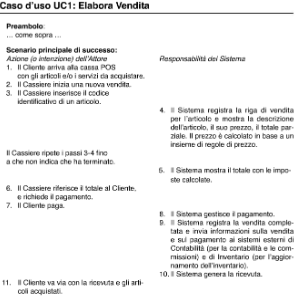
\includegraphics[scale = 0.65]{images/Notazione.png}} 
        \subfloat[Relativa tabella]{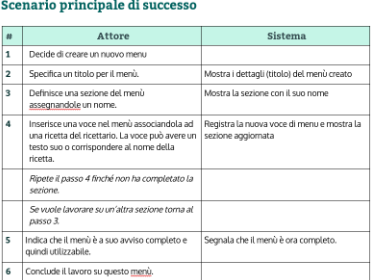
\includegraphics[scale = 0.65]{images/Notazione2.png}}
    \end{figure}
    \item [$\Rightarrow$] Le estensioni vanno indicate con riferimento al passo dello scenario principale.
\begin{figure}[!h]
    \centering
    \subfloat[Estensione del punto 1]{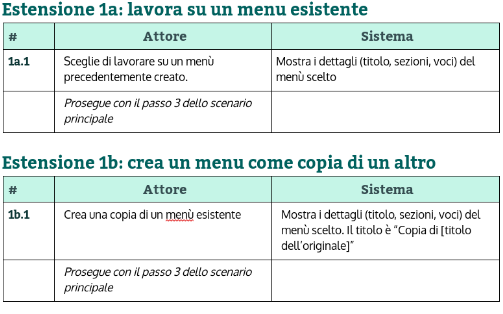
\includegraphics[scale = 0.4]{images/Estensione1.png}} 
    \subfloat[Estensione del punto 3]{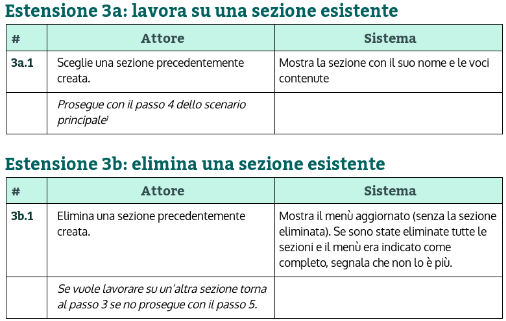
\includegraphics[scale = 0.4]{images/Estensione2.png}}
\end{figure}
\item [$\Rightarrow$] Ci possono essere alternative che possono occorrere in più passi.
\begin{figure}[!h]
    \centering
    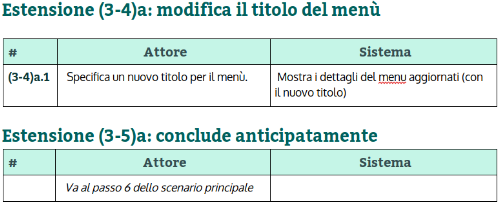
\includegraphics[scale = 0.55]{images/Estensione3.png}
\end{figure}
\end{itemize}

\ex{Passi ed estensioni}{
    \begin{center}
        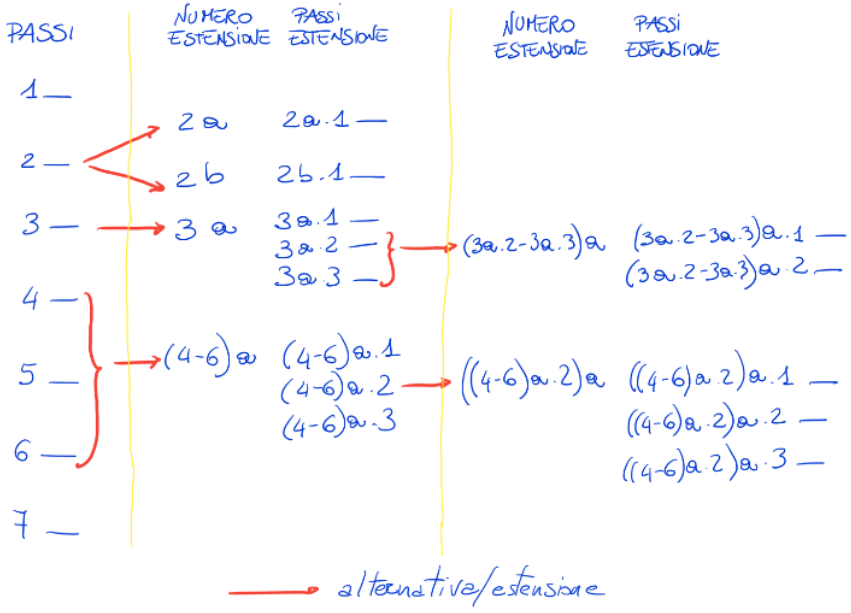
\includegraphics[scale = 0.4]{images/Passi ed estensioni.png}
    \end{center}
}

\nt{Lo stile deve essere \newfancyglitter{essenziale} e \newfancyglitter{coinciso}. Si ignora l'interfaccia utente, ci si concentra sull'Obiettivo Utente.}

\dfn{Stile essenziale}{
    La narrativa è espressa a livello di \newfancyglitter{intenzioni} e 
    \newfancyglitter{responsabilità}, non con riferimento ad azioni concrete.
    Le intenzioni e le responsabilità devono rimanere indipendenti dai dettagli tecnologici e dagli attori.
}

\ex{Stile}{
    \begin{itemize}
        \item [\textcolor{dkgreen}{\checkmark}] L'Amministratore si identifica.
        \item [\textcolor{dkgreen}{\checkmark}] Il Sistema autentica l'identità.
        \item [\textcolor{red}{\XSolidBrush}] L'Amministratore inserisce ID e password nella finestra di dialogo.
        \item [\textcolor{red}{\XSolidBrush}] Il sistema autentica l'Amministratore.
        \item [\textcolor{red}{\XSolidBrush}] Il sistema visualizza la finestra "edit users".
    \end{itemize}
}

\nt{Durante l'analisi dei requisiti bisogna specificare il comportamento
esterno del Sistema, considerato a "scatola nera". Non bisogna prendere decisioni
sul "come".

\begin{itemize}
    \item [\textcolor{red}{\XSolidBrush}] Il Sistema memorizza la vendita in una base di dati.
    \item [\textcolor{red}{\XSolidBrush}] Il Sistema esegue un'istruzione SQL INSERT per la vendita.
\end{itemize}
}

\subsection{Trovare i Casi d'Uso}

\begin{enumerate}
    \item Scegliere i confini del Sistema;
    \item Identificare gli attori primari;
    \item Identificare gli obiettivi di ciascun attore primario;
    \item Definire i Casi d'Uso che soddisfano gli obiettivi degli utenti.
\end{enumerate}

\ex{Identificare gli attori primari}{
    \begin{center}
        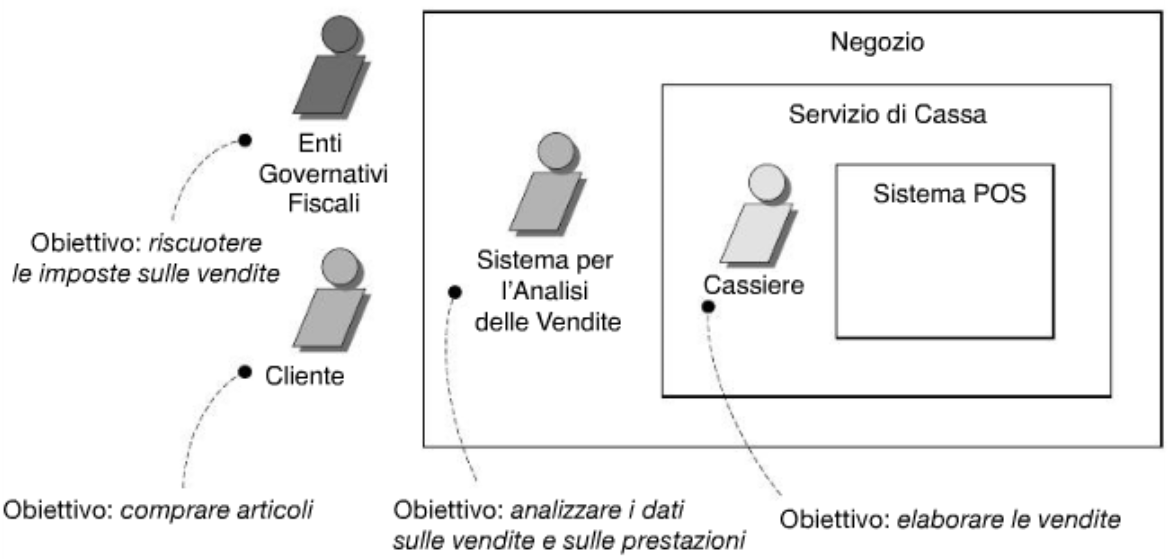
\includegraphics[scale = 0.3]{images/Identificare gli attori primari.png}
        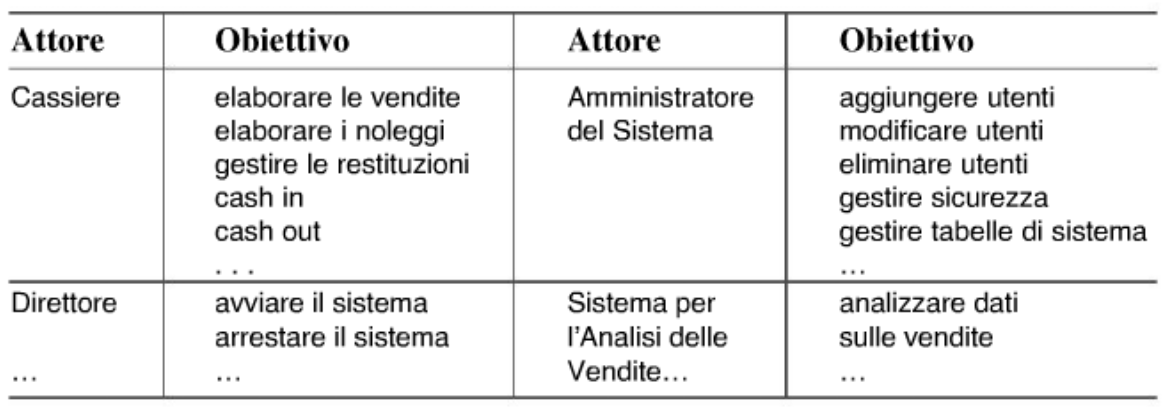
\includegraphics[scale = 0.3]{images/Identificare gli attori 2.png}
    \end{center}

}

\qs{}{Qual è un livello utile per esprimere i Casi d'Uso nell'analisi dei requisiti di un'applicazione software?}
\begin{itemize}
    \item [$\Rightarrow$] Il test del \fancyglitter{capo}: il capo sarà felice?
    \item [$\Rightarrow$] Il test \fancyglitter{EBP} (Elementary Business Process): un processo di Business è un'attività che aggiunge un valore;
    \item [$\Rightarrow$] Il test della \fancyglitter{dimensione}: un Caso d'Uso raramente richiede una singola azione o passo. Normalmente, nella forma dettagliata, richiede dalle 3 alle 10 pagine.
\end{itemize}

\ex{Verificare l'utilità dei Casi d'Uso}{
    \begin{itemize}
        \item \textcolor{red}{\XSolidBrush} Negoziare un contratto con un fornitore.
        \begin{itemize}
            \item [$\Rightarrow$] Troppo grande.

        \end{itemize}
        \item \textcolor{dkgreen}{\checkmark} Gestire una restituzione.
        \begin{itemize}
            \item [$\Rightarrow$] D'accordo con il capo, simile a EBP, dimensioni adeguate.
        \end{itemize}
        \item \textcolor{red}{\XSolidBrush} Effetture il login.
        \begin{itemize}
            \item [$\Rightarrow$] Il capo non è contento se ci si limita a fare solo quello tutta la giornata.
        \end{itemize}
        \item \textcolor{red}{\XSolidBrush} Spostare una pedina sul tabellone da gioco.
        \begin{itemize}
            \item [$\Rightarrow$] Passo singolo, non supera il test della dimensione.
        \end{itemize}
    \end{itemize}
}

\subsection{Livello dei Casi d'Uso}

\dfn{Livello di obiettivo utente}{
    Nell'analisi dei requisiti è utile concentrarsi sui casi utente EBP.
}

\dfn{Livello di sotto-funzione}{
    Rappresenta una funzionalità nell'uso del sistema.
    Utile per mettere a fattor comune sequenze di passi condivise da più Casi
    d'Uso, evitando duplicazione di testo.
}

\ex{Diagramma dei Casi d'Uso (UCD)}{
    \begin{center}
        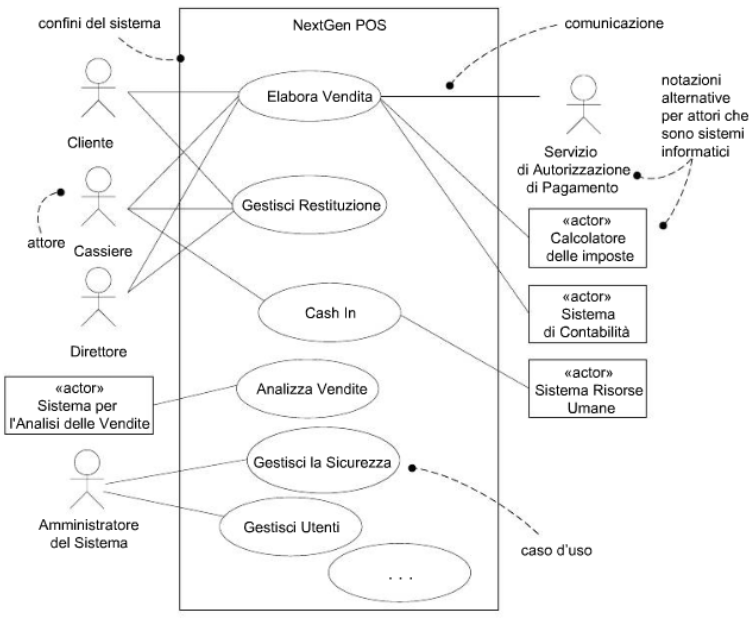
\includegraphics[scale = 0.5]{images/UCD.png}
    \end{center}

}
\section{Elaborazione}

\dfn{Elaborazione}{
    L'elaborazione è la serie iniziale di iterazioni durante le quali il team
    esegue un'indagine seria, implementa il nucleo dell'architettura,
    chiarisce la maggior parte dei requisiti e affronta le problematiche
    più rischiose.
}

\nt{Durante questa fase vengono creati prototipi "usa e getta" ma codice
e progettazione sono parti di qualità-produzione del sistema finale.}
\pagebreak
\subsection{Pianificazione dell'iterazione successiva}

I requisiti e le iterazioni sono organizzate in base a:

\begin{itemize}
    \item [$\Rightarrow$] \fancyglitter{Rischio}: tecnico, incertezza dello sforzo, usabilità;
    \item [$\Rightarrow$] \fancyglitter{Copertura}: le iterazioni iniziali devono coprire tutte le parti principali del sistema;
    \item [$\Rightarrow$] \fancyglitter{Criticità}: le funzioni che il cliente ritiene più importanti.
\end{itemize}

\nt{La classifica viene stilata prima dell'iterazione 1, poi prima dell'iterazione 2 e così via. La lista non è definitiva.

\begin{center}
    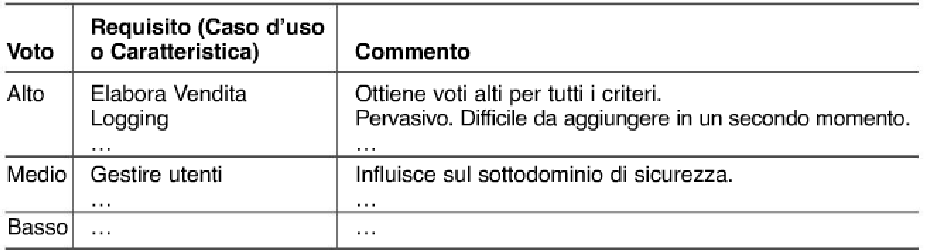
\includegraphics[scale=0.5]{images/Classifica.png}
\end{center}
}

\dfn{Iterazione 1}{
    Nell'iterazione 1 si implementa un sottoinsieme dei requisiti o dei Casi d'Uso completi.
}

\subsection{Artefatti dell'Elaborazione}

\begin{center}
    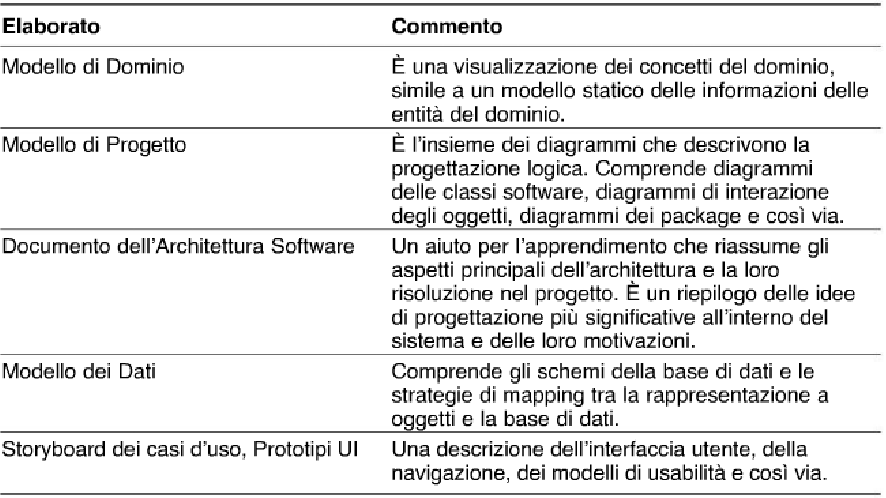
\includegraphics[scale=0.5]{images/Artefatti elaborazione.png}
\end{center}

\begin{center}
    
\end{center}

\section{Modello di Dominio}

\section{Diagrammi di sequenza del sistema (DSS)}

\section{Contratti}
\label{contratti}